\documentclass[12pt]{report}
\usepackage[a4paper, margin=1in]{geometry}
\usepackage{qrcode}
\usepackage{graphicx}
\usepackage{hyperref}
\usepackage{listings}
\usepackage{amsmath}
\usepackage{amssymb}
\usepackage{float}
\title{Car Database Management System}
\author{
  Abhishek Gupta \\ 
  Samuel Koshey \\ 
  Jaydeep Roy \\ 
  Krutik Vanjara
}
\begin{document}

\maketitle
\tableofcontents
\newpage

\chapter*{Abstract}
\addcontentsline{toc}{chapter}{Abstract}
This project focuses on designing, securing, optimizing, and automating the management of an Information System for a used car dataset. It includes preparing a relational schema, implementing security measures, optimizing queries, and automating tasks. Furthermore, the dataset serves as a basis for machine learning applications, including price prediction with linear regression.

\chapter{Introduction}
Managing information systems for used cars can be complex due to the diverse nature of the data and the need for security, optimization, and automation. This project organizes the data using a relational schema, enforces security policies, optimizes queries for efficient data retrieval, and provides a graphical interface for end-user interaction. 

\section{Dataset Details}
The dataset used in this project is sourced from \href{https://www.kaggle.com/datasets/nehalbirla/vehicle-dataset-from-cardekho?select=car+details+v4.csv}{Kaggle}. It includes the following columns:
\begin{itemize}
    \item \texttt{name}
    \item \texttt{year}
    \item \texttt{selling\_price}
    \item \texttt{km\_driven}
    \item \texttt{fuel}
    \item \texttt{seller\_type}
    \item \texttt{transmission}
    \item \texttt{Owner}
\end{itemize}

The dataset is provided as five CSV files.

\chapter{Relational Schema}
The relational schema for the database is designed to store information across five primary tables:

\section{Entities}
\begin{enumerate}
    \item\textbf{Entities:}
    \begin{itemize}
        \item \texttt{Cars}
        \item \texttt{Features}
        \item \texttt{Specifications}
        \item \texttt{Dimensions}
        \item \texttt{Ownership}
    \end{itemize}
    \end{enumerate}
    \section{Tables}
    \begin{enumerate}
     \item \textbf{Cars Table:}
    \begin{itemize}
        \item \texttt{CAR\_ID (Primary Key)}
        \item \texttt{MAKE}
        \item \texttt{MODEL}
        \item \texttt{PRICE}
        \item \texttt{YEAR}
        \item \texttt{FUEL\_TYPE}
        \item \texttt{LOCATION}
        \item \texttt{TRANSMISSION}
    \end{itemize}

    \item \textbf{Features Table:}
    \begin{itemize}
        \item \texttt{FEATURE\_ID (Primary Key)}
        \item \texttt{CAR\_ID (Foreign Key)}
        \item \texttt{COLOR}
        \item \texttt{SEATING\_CAPACITY}
        \item \texttt{FUEL\_TANK\_CAPACITY}
    \end{itemize}

    \item \textbf{Specifications Table:}
    \begin{itemize}
        \item \texttt{SPEC\_ID (Primary Key)}
        \item \texttt{CAR\_ID (Foreign Key)}
        \item \texttt{ENGINE}
        \item \texttt{MAX\_POWER}
        \item \texttt{MAX\_TORQUE}
        \item \texttt{DRIVETRAIN}
    \end{itemize}

    \item \textbf{Dimensions Table:}
    \begin{itemize}
        \item \texttt{DIMENSION\_ID (Primary Key)}
        \item \texttt{CAR\_ID (Foreign Key)}
        \item \texttt{LENGTH}
        \item \texttt{WIDTH}
        \item \texttt{HEIGHT}
    \end{itemize}

    \item \textbf{Ownership Table:}
    \begin{itemize}
        \item \texttt{OWNERSHIP\_ID (Primary Key)}
        \item \texttt{CAR\_ID (Foreign Key)}
        \item \texttt{OWNER}
        \item \texttt{SELLER\_TYPE}
        \item \texttt{KILOMETER}
    \end{itemize}
\end{enumerate}
\section{Constraints:}
\begin{table}[h]  
    \centering  
    \caption{Constraints}
    \begin{tabular}{|l|l|l|}  
        \hline  
        \textbf{Constraint Name} & \textbf{Constraint Type} & \textbf{Search Condition} \\ \hline  
        CHK\_PRICE                & Check                    & Price $\geq$ 0                \\ \hline  
        CHK\_YEAR                 & Check                    & Year BETWEEN 1886 AND 9999\\ \hline  
        SYS\_C008363              & Primary Key              & (null)                    \\ \hline  
        SYS\_C008364              & Check                    & CAR\_ID IS NOT NULL      \\ \hline  
        SYS\_C008365              & Check                    & MAKE IS NOT NULL        \\ \hline  
        SYS\_C008366              & Check                    & MODEL IS NOT NULL       \\ \hline  
        SYS\_C008367              & Check                    & PRICE IS NOT NULL       \\ \hline  
        SYS\_C008368              & Check                    & YEAR IS NOT NULL        \\ \hline  
        SYS\_C008369              & Check                    & FUEL\_TYPE IS NOT NULL   \\ \hline  
        SYS\_C008370              & Check                    & LOCATION IS NOT NULL    \\ \hline  
        SYS\_C008371              & Check                    & TRANSMISSION IS NOT NULL \\ \hline  
    \end{tabular}  
\end{table}
\chapter{Security and User Management}
\section{Overview}  
This section details user and role management in the car management system, ensuring appropriate access levels to database tables for different users. The system accommodates three user types: admin, manager, and regular users, each with distinct roles and permissions.  
\section{Users and Roles}  
\begin{enumerate}
   \item \textbf{Admin User (C\#\#admin\_user)}  
    \begin{itemize}  
        \item \textbf{Role:} C\#\#admin\_role  
        \item \textbf{Permissions:} Full access to all tables (CarDetails, CarSpecifications, CarFeatures, CarOwnership, CarDimensions).  
    \end{itemize}
    \item \textbf{Manager User (C\#\#manager\_user)}  
    \begin{itemize}  
        \item \textbf{Role:} C\#\#manager\_role  
        \item \textbf{Permissions:} Modify access (read, insert, update) to all tables, with no Data Definition Language (DDL) permissions.  
    \end{itemize}  
    
    \item \textbf{Regular User (C\#\#regular\_user)}  
    \begin{itemize}  
        \item \textbf{Role:} C\#\#regular\_role  
        \item \textbf{Permissions:} Read-only access to all tables.  
    \end{itemize}  
\end{enumerate}

\section{Role Creation and Privileges}  

\begin{itemize}  
    \item \textbf{Admin Role (C\#\#admin\_role):} Full access to all tables.  
    \item \textbf{Manager Role (C\#\#manager\_role):} Select, insert, and update privileges on all tables.  
    \item \textbf{Regular Role (C\#\#regular\_role):} Select privileges on all tables.  
\end{itemize}  

\section{Assigning Roles to Users}  

\begin{itemize}  
    \item C\#\#admin\_role is assigned to C\#\#admin\_user.  
    \item C\#\#manager\_role is assigned to C\#\#manager\_user.  
    \item C\#\#regular\_role is assigned to C\#\#regular\_user.  
\end{itemize}  

\section{Password Policy}  
The default profile is modified to set a 90-day password lifetime, requiring periodic password changes.  

\section{Views for Restricted Access}  
A view, \texttt{CarDetails\_View}, is created to limit access to specific columns (Car\_ID, Make, Model) for users with the C\#\#regular\_role, ensuring the underlying table remains secure by restricting access to other columns.  

\chapter{Queries and Optimization}
This section demonstrates SQL queries for data retrieval and optimization, including car listings, average price calculations, and query performance improvements. Optimized queries are documented in the project repository \href{Optimized_result.pdf}{here}.

\begin{figure}[H]
    \centering
    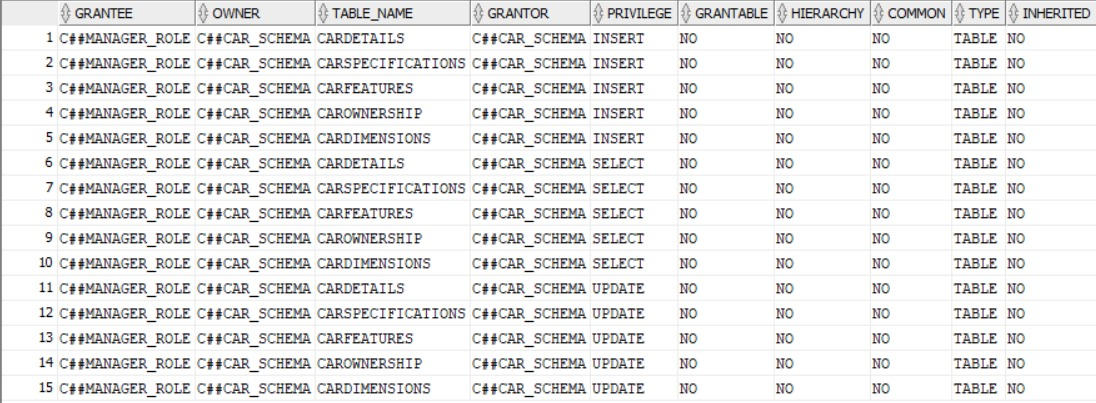
\includegraphics[width=0.8\textwidth]{g3.jpg}
    \caption{Optimization of query}
\end{figure}

\chapter{Automation}
\section{Overview}
Automation in this project includes triggers, functions, and procedures for managing and streamlining database operations. Examples include:
\begin{itemize}
    \item Logging deletions.
    \item Restricting unauthorised actions.
    \item Calculating total car values.
    \item Counting cars based on criteria.
\end{itemize}

\chapter{Graphical Interface}
\section{Overview}
Two GUI applications, \texttt{gui\_system.py} and \texttt{Bonus.py}, were developed using Python's Tkinter and cx\_Oracle libraries for dynamic car data management. Features include:
\begin{itemize}
    \item Dynamic filtering with dropdown menus.
    \item Real-time query execution.
    \item CSV export functionality.
\end{itemize}

\section{Screenshots}
\begin{figure}[H]
    \centering
    \includegraphics[width=0.8\textwidth]{g1.jpg}
    \caption{Graphical Interface Example 1}
\end{figure}
\begin{figure}[H]
    \centering
    \includegraphics[width=0.8\textwidth]{g2.jpg}
    \caption{Graphical Interface Example 2}
\end{figure}

\chapter{Conclusion}
This project effectively showcases the design, security, optimization, and automation of a car management database, enhanced by user-friendly GUIs for non-technical users. Future developments will focus on expanding machine learning capabilities for price prediction.The integration of robust data protection measures ensures that sensitive information remains secure while still being accessible to authorized personnel. Additionally, the optimization of database queries and indexing techniques significantly enhances the performance of the system, allowing for swift data retrieval and processing. 

To further streamline operational efficiency, various automation features have been implemented, such as scheduled maintenance reminders and automated reporting tools, saving time and minimizing human error. The user interfaces have been meticulously designed with intuitive navigation and clear visual cues, enabling users from diverse backgrounds to interact with the database confidently.

In the upcoming phases of development, our attention will pivot towards leveraging machine learning algorithms to provide insightful analytics and predictive modeling. This exciting direction will empower users not only to forecast pricing trends but also to evaluate factors influencing car demand and market dynamics. 

Overall, this project lays a solid foundation for future enhancements, positioning itself as a vital resource in the automotive industry. With continuous feedback integration and iterative improvements, we aim to cultivate an adaptive and intelligent car management system that meets the evolving needs of our users.



\begin{center}  
    \qrcode{https://github.com/Krutik-Vanjara/VEHICLE_DATABASE/tree/main} % Replace with your actual GitHub repo link  
    \vspace{20pt}  
    \textbf{Scan to access our GitHub repository!}  
\end{center}  

\end{document}

